
\chapter{Mathematics}

\section{Master Theorem}
\begin{equation*}
    T(n) = 
        \begin{cases}
            aT(\frac{n}{b}) + \Theta(n^c) & n > n_0\\
            \Theta(1) & n \leq n_0
        \end{cases}
\end{equation*}

\begin{itemize}
  \item $c > \log_ba : T(n) = \Theta(n^c)$
  \item $c = \log_ba : T(n) = \Theta(n^c\log n)$
  \item $c < \log_ba : T(n) = \Theta(n^{\log_ba})$
\end{itemize}

\section{Equations}
\[ax^2+bx+c=0 \Rightarrow x = \frac{-b\pm\sqrt{b^2-4ac}}{2a}\]

The extremum is given by $x = -b/2a$.

\[\begin{aligned}ax+by=e\\cx+dy=f\end{aligned}
\Rightarrow
\begin{aligned}x=\dfrac{ed-bf}{ad-bc}\\y=\dfrac{af-ec}{ad-bc}\end{aligned}\]

In general, given an equation $Ax = b$, the solution to a variable $x_i$ is given by
\[x_i = \frac{\det A_i'}{\det A} \]
where $A_i'$ is $A$ with the $i$'th column replaced by $b$.

\section{Recurrences}
If $a_n = c_1 a_{n-1} + \dots + c_k a_{n-k}$, and $r_1, \dots, r_k$ are distinct roots of $x^k - c_1 x^{k-1} - \dots - c_k$, there are $d_1, \dots, d_k$ s.t.
\[a_n = d_1r_1^n + \dots + d_kr_k^n. \]
Non-distinct roots $r$ become polynomial factors, e.g. $a_n = (d_1n + d_2)r^n$.

\section{Trigonometry}
\begin{align*}
\sin(v+w)&{}=\sin v\cos w+\cos v\sin w\\
\cos(v+w)&{}=\cos v\cos w-\sin v\sin w\\
\end{align*}
\begin{align*}
\tan(v+w)&{}=\dfrac{\tan v+\tan w}{1-\tan v\tan w}\\
\sin v+\sin w&{}=2\sin\dfrac{v+w}{2}\cos\dfrac{v-w}{2}\\
\cos v+\cos w&{}=2\cos\dfrac{v+w}{2}\cos\dfrac{v-w}{2}
\end{align*}
\[ (V+W)\tan(v-w)/2{}=(V-W)\tan(v+w)/2 \]
where $V, W$ are lengths of sides opposite angles $v, w$.
\begin{align*}
	a\cos x+b\sin x&=r\cos(x-\phi)\\
	a\sin x+b\cos x&=r\sin(x+\phi)
\end{align*}
where $r=\sqrt{a^2+b^2}, \phi=\operatorname{atan2}(b,a)$.

\section{Geometry}

\subsection{Triangles}
Side lengths: $a,b,c$\\
Semiperimeter: $p=\dfrac{a+b+c}{2}$\\
Area: $A=\sqrt{p(p-a)(p-b)(p-c)}$\\
Circumradius: $R=\dfrac{abc}{4A}$\\
Inradius: $r=\dfrac{A}{p}$\\
Length of median (divides triangle into two equal-area triangles): $m_a=\tfrac{1}{2}\sqrt{2b^2+2c^2-a^2}$\\
Length of bisector (divides angles in two): $s_a=\sqrt{bc\left[1-\left(\dfrac{a}{b+c}\right)^2\right]}$\\
Law of sines: $\dfrac{\sin\alpha}{a}=\dfrac{\sin\beta}{b}=\dfrac{\sin\gamma}{c}=\dfrac{1}{2R}$\\
Law of cosines: $a^2=b^2+c^2-2bc\cos\alpha$\\
Law of tangents: $\dfrac{a+b}{a-b}=\dfrac{\tan\dfrac{\alpha+\beta}{2}}{\tan\dfrac{\alpha-\beta}{2}}$\\

\subsection{Quadrilaterals}
With side lengths $a,b,c,d$, diagonals $e, f$, diagonals angle $\theta$, area $A$ and
magic flux $F=b^2+d^2-a^2-c^2$:

\[ 4A = 2ef \cdot \sin\theta = F\tan\theta = \sqrt{4e^2f^2-F^2} \]

 For cyclic quadrilaterals the sum of opposite angles is $180^\circ$,
$ef = ac + bd$, and $A = \sqrt{(p-a)(p-b)(p-c)(p-d)}$.

\subsection{Spherical coordinates}
\begin{center}
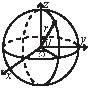
\includegraphics[width=25mm]{Math/sphericalCoordinates}
\end{center}
\[\begin{array}{cc}
x = r\sin\theta\cos\phi & r = \sqrt{x^2+y^2+z^2}\\
y = r\sin\theta\sin\phi & \theta = \textrm{acos}(z/\sqrt{x^2+y^2+z^2})\\
z = r\cos\theta & \phi = \textrm{atan2}(y,x)
\end{array}\]

\section{Derivatives/Integrals}
\begin{align*}
	\dfrac{d}{dx}\arcsin x = \dfrac{1}{\sqrt{1-x^2}} &&& \dfrac{d}{dx}\arccos x = -\dfrac{1}{\sqrt{1-x^2}} \\
	\dfrac{d}{dx}\tan x = 1+\tan^2 x &&& \dfrac{d}{dx}\arctan x = \dfrac{1}{1+x^2} \\
	\int\tan ax = -\dfrac{\ln|\cos ax|}{a} &&& \int x\sin ax = \dfrac{\sin ax-ax \cos ax}{a^2} \\
	\int e^{-x^2} = \frac{\sqrt \pi}{2} \text{erf}(x) &&& \int xe^{ax}dx = \frac{e^{ax}}{a^2}(ax-1)
\end{align*}

Integration by parts:
\[\int_a^bf(x)g(x)dx = [F(x)g(x)]_a^b-\int_a^bF(x)g'(x)dx\]

\section{Sums}
\[ c^a + c^{a+1} + \dots + c^{b} = \frac{c^{b+1} - c^a}{c-1}, c \neq 1 \]
\begin{align*}
	1 + 2 + 3 + \dots + n &= \frac{n(n+1)}{2} \\
	1^2 + 2^2 + 3^2 + \dots + n^2 &= \frac{n(2n+1)(n+1)}{6} \\
	1^3 + 2^3 + 3^3 + \dots + n^3 &= \frac{n^2(n+1)^2}{4} \\
	1^4 + 2^4 + 3^4 + \dots + n^4 &= \frac{n(n+1)(2n+1)(3n^2 + 3n - 1)}{30} \\
\end{align*}

\section{Series}
$$e^x = 1+x+\frac{x^2}{2!}+\frac{x^3}{3!}+\dots,\,(-\infty<x<\infty)$$
$$\ln(1+x) = x-\frac{x^2}{2}+\frac{x^3}{3}-\frac{x^4}{4}+\dots,\,(-1<x\leq1)$$
$$\sqrt{1+x} = 1+\frac{x}{2}-\frac{x^2}{8}+\frac{2x^3}{32}-\frac{5x^4}{128}+\dots,\,(-1\leq x\leq1)$$
$$\sin x = x-\frac{x^3}{3!}+\frac{x^5}{5!}-\frac{x^7}{7!}+\dots,\,(-\infty<x<\infty)$$
$$\cos x = 1-\frac{x^2}{2!}+\frac{x^4}{4!}-\frac{x^6}{6!}+\dots,\,(-\infty<x<\infty)$$

\section{Probability theory}
Let $X$ be a discrete random variable with probability $p_X(x)$ of assuming the value $x$. It will then have an expected value (mean) $\mu=\mathbb{E}(X)=\sum_xxp_X(x)$ and variance $\sigma^2=V(X)=\mathbb{E}(X^2)-(\mathbb{E}(X))^2=\sum_x(x-\mathbb{E}(X))^2p_X(x)$ where $\sigma$ is the standard deviation. If $X$ is instead continuous it will have a probability density function $f_X(x)$ and the sums above will instead be integrals with $p_X(x)$ replaced by $f_X(x)$.

Expectation is linear:
\[\mathbb{E}(aX+bY) = a\mathbb{E}(X)+b\mathbb{E}(Y)\]
For independent $X$ and $Y$, \[V(aX+bY) = a^2V(X)+b^2V(Y).\]

\section{Generating functions}

Example of finding generating functions:

$a_0=1$

$a_1=2$

$a_n=6a_{n-1}-8a_{n-2}+n, n\geq2$

$G(z)=a_0+a_1z+\sum\limits_{n=2}^{\infty}(6a_{n-1}-8a_{n-2}+n)z^n$

$G(z)=a_0+a_1z+6\sum\limits_{n=2}^{\infty}a_{n-1}z^n-8\sum\limits_{n=2}^{\infty}a_{n-2}z^n+\sum\limits_{n=2}^{\infty}nz^n$

$G(z)=a_0+a_1z+6z\sum\limits_{n=1}^{\infty}a_{n}z^n-8z^2\sum\limits_{n=0}^{\infty}a_{n}z^n+\sum\limits_{n=2}^{\infty}nz^n$


$G(z)=a_0+a_1z+6z(G(z) - a_0)-8z^2G(z)+\sum\limits_{n=2}^{\infty}nz^n$


$G(z)=1-4z+6zG(z)-8z^2G(z)+\sum\limits_{n=2}^{\infty}nz^n$  


To calculate $\sum\limits_{n=2}^{\infty}nz^n$ use generating function $B(z)$ for $b_n=(1,1,1,1,...)$ :

$zB'(z)=z(\sum\limits_{n=0}^{\infty}b_nz^n)'=\sum\limits_{n=0}^{\infty}b_nz^n$

Then we can do:

$\sum\limits_{n=2}^{\infty}nz^2=z\sum\limits_{n=2}^{\infty}nz^{n-1}=z(\sum\limits_{n=2}^{\infty}z^n)'$

$\sum\limits_{n=2}^{\infty}z^n=\sum\limits_{n=0}^{\infty}z^n-1-z=\frac{1}{1-z}-1-z=\frac{z^2}{1-z}$

$z(\frac{z^2}{1-z})'=\frac{z^2(2-z)}{(1-z)^2}$

Then:

$G(z)=1-4z+6zG(z)-8z^22G(z)+\frac{z^2(2-z)}{(1-z)^2}$

$G(z)=\frac{1-6z+11z^2-5z^3}{(1-6z+8z^2)(1-z)^2}$

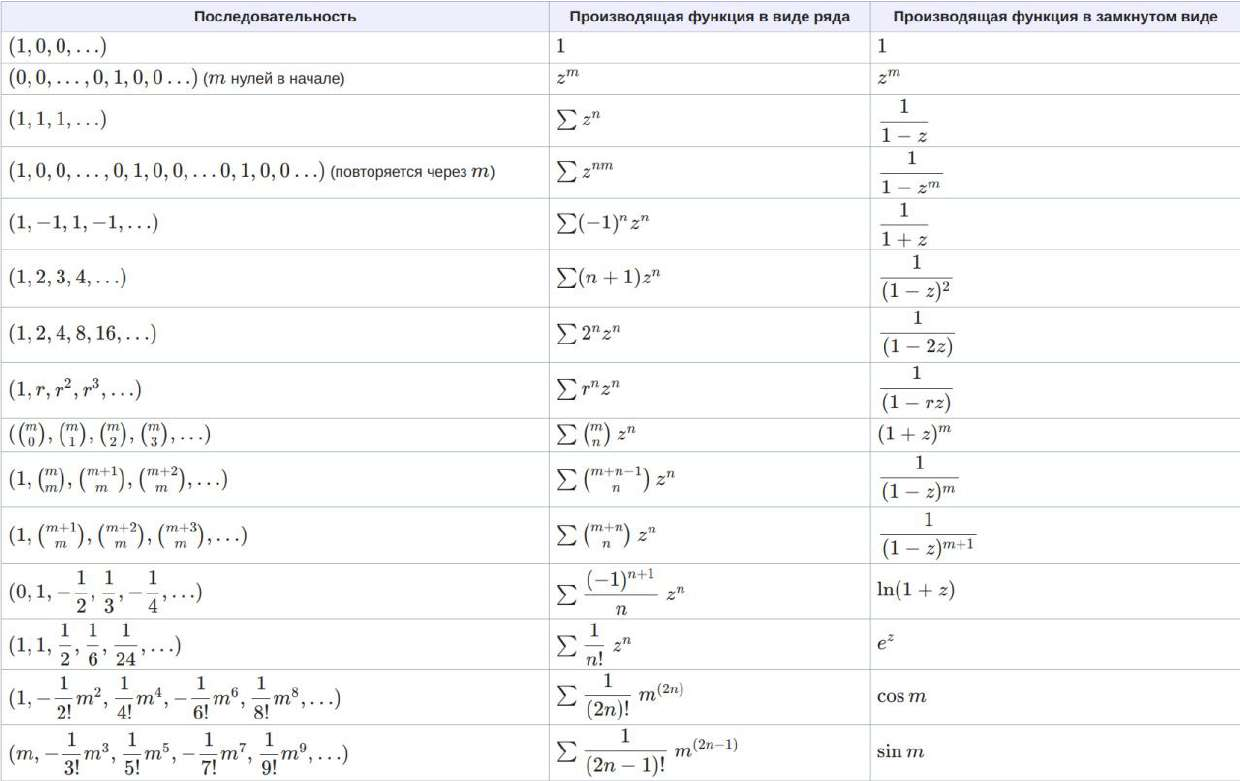
\includegraphics[width=80mm]{Math/generatingFunctions}